\chapter{Background}
\label{c:Background}

\section{Program Comprehension}

\begin{figure}[tb]
	\centering
	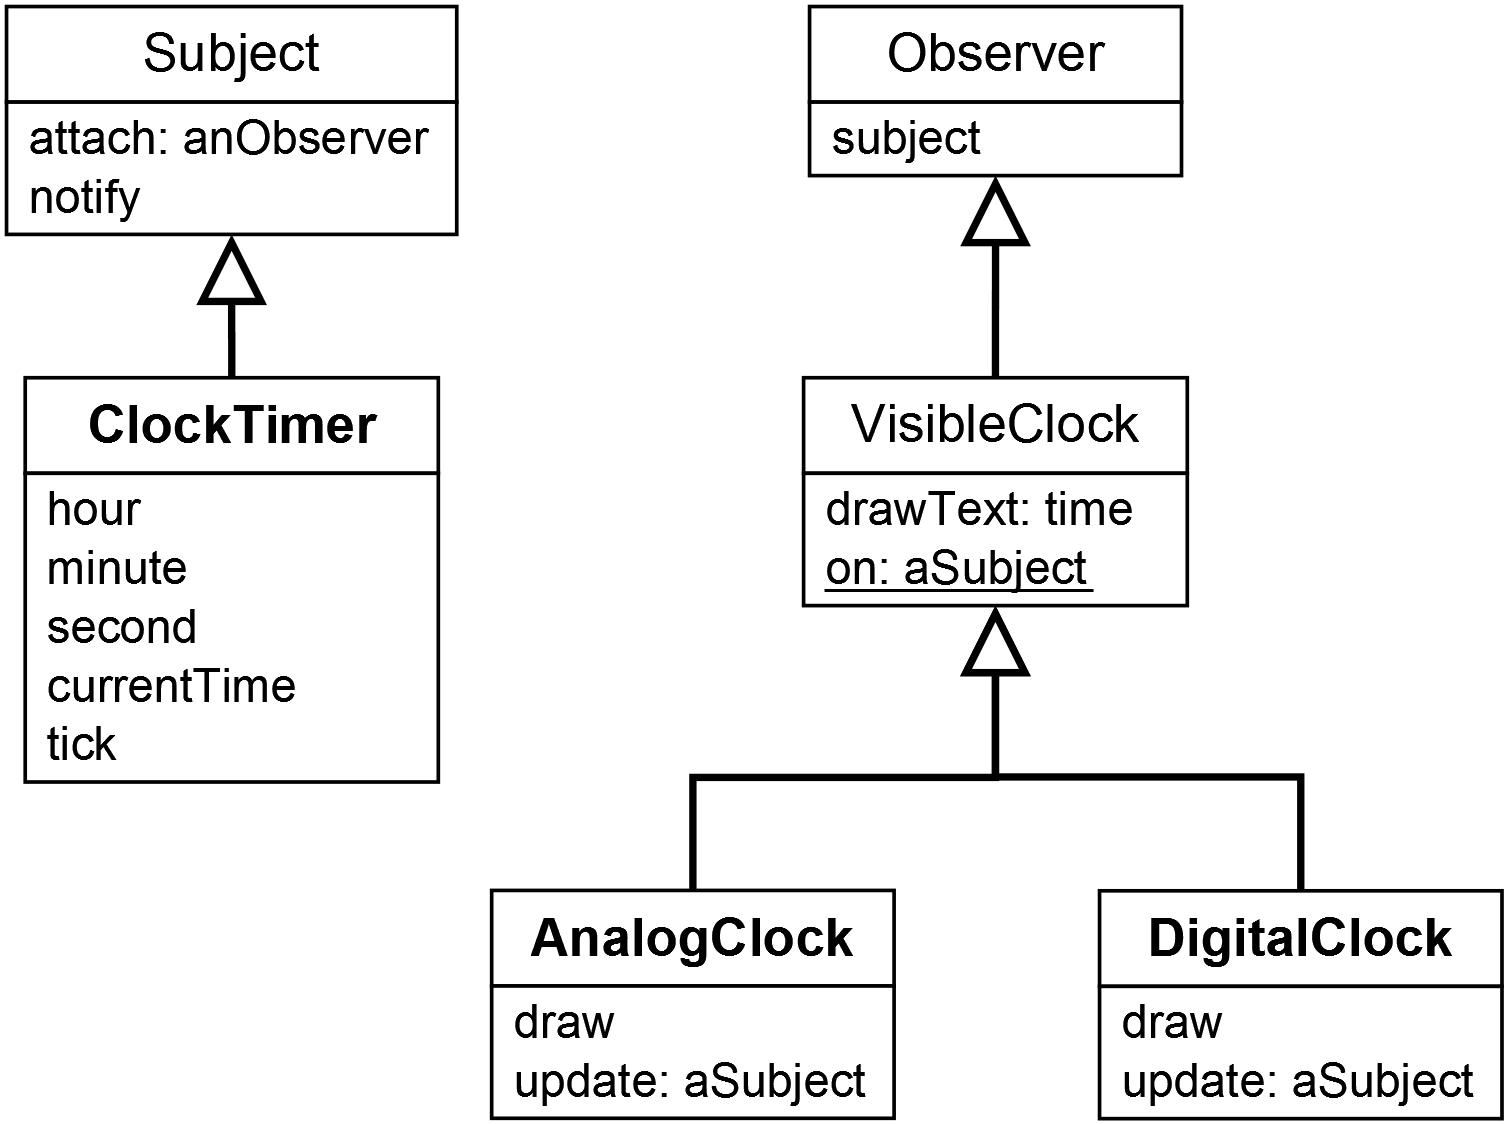
\includegraphics[width=0.7\textwidth]{../images/02-ObserverExample}
	\caption[foo]{Foo}
	\label{fig:ObserverExample}
\end{figure}

Throughout the following chapters, the manifestation of the observer pattern \cite{gamma_design_1995} that is depicted in Figure \ref{fig:ObserverExample} will serve as an illustrating example.
The component that emits events and thus functions as the \inlinecode{Subject} is a clock timer.
It has internal state describing the current time and provides various accessors to this state.
In addition, an interface which allows to increment the clock timer is exposed through the \inlinecode{tick} method.

Several clock visualizations can act as observers of this clock timer.
Their common base class is \inlinecode{VisibleClock}, which provides a factory method \cite{gamma_design_1995} and implements the drawing of clocks through a template method \cite{gamma_design_1995}.
\inlinecode{AnalogClock} and \inlinecode{DigitalClock} provide two different visualizations for clock timers in analog and digital fashion.
Therefore, they implement the \inlinecode{draw} method which is a part of the template method \inlinecode{drawText:}.
Furthermore, they provide an interface for subject notifications through the \inlinecode{update:} method.

The components form a pull-observer pattern, meaning that subjects notify observers of changes, but do not pass the new state along with the notification.
All observers have to pull required information from the subject on notifications. 

\section{Dynamic Analysis: A Necessary Evil}
\label{s:BackgroundAnalysis}

\subsection{The Need for Dynamic Analysis}
Program comprehension usually is facilitated through two different analysis techniques, namely static and dynamic analysis.
Static analysis is executed solely with the help of source code entities.
Common examples of information that can be derived via such analyses are inheritance relationships and metrics like cyclomatic complexity or lines of code.
Furthermore, lint-tools and static code verifiers fall within the same category.
Static program analysis has two advantages.
First, it is complete in the sense that all of the source code can be considered, and thus all possible executions of a program are covered by an analysis.
Second, many static analyses can be performed rapidly.
However, this factor is largely dependent on the deepness of the analysis, and especially in the case of formal verification tools runtime is an issue \cite{wichmann_industrial_1995}.

However, when it comes to the analysis of objects and their interactions, information is required that no longer can be derived from the source code alone.
Due to object oriented concepts like polymorphism and late binding, the concrete manifestation of static source code entities is only known at runtime.
Object-oriented code defines classes and their relationships rather than collaborations of objects, which are spread throughout the code.
Furthermore, polymorphism can hide which classes actually get instantiated at runtime.
The consequence is a huge gap between the structure of the source code, and the runtime structure of programs that consists of a network of collaborating objects.
Gamma et al. use the following analogy to describe this disparity:

\begin{quote}
Trying to understand one from the other is like trying to understand the dynamism of living ecosystems from the static taxonomy of plants and animals, and vice-versa.
\par\raggedleft--- \textup{Gamma et al.}, \cite{gamma_design_1995}
\end{quote}

Consequently, it is inevitable to investigate the properties of a running system in order to draw conclusions about objects and their interactions.
This procedure is known as dynamic analysis.

Dynamic analysis has the advantage that it is goal-oriented, meaning that specific scenarios can be executed and analyzed that cover the functionality the developer is interested in.
Furthermore, it is precise in the sense that polymorphic method calls and late binding can be resolved.
However, this comes at the cost of completeness, since dynamic analysis never can cover any possible behavior of a software system, but only that displayed during the analyzed execution.
Apart from that, dynamic analysis suffers from four major scalability issues that are presented in the following section.

\subsection{The Four Problems of Dynamic Analysis}

\subsubsection{Execution Time}
In order to get an insight into the behavior of a software system at runtime, the execution of said system has to be recorded somehow.
The most common approach for this purpose is instrumentation, which can be done at the source code or byte code level.
In this process, code is automatically added to the program under observation before its execution.
For instance, this could be tracing calls before and after every method execution which subsequently record the methods that get executed and their chronological order.

Another common strategy is to exploit debug interfaces to simulate the execution of a program.
For instance, the Java Virtual Machine Debug Interface (JVMDI) can be utilized to step through a program automatically.
At the same time, the internal state of the program can be inspected.
Thus, a trace of the call stack and of the effects of method executions on program state can be recorded.

Less common approaches in the field of dynamic program analysis are sampling techniques, which are usually used for performance measurements, and tracing at the level of the virtual machine.

But regardless of the strategy that is chosen, all these approaches slow down the execution of the system under observation massively.
Instrumented program executions are reported to be 15 up to over 100 times slower compared to undisturbed executions \cite{pothier_scalable_2007, karran_synctrace:_2013}.
For instance, Karran reports that the instrumented execution of the Firefox browser and the subsequent loading of a Google search result page take up to two minutes \cite{karran_extraction_2013}.

As a consequence, developers have to wait a long time for the generation of an execution trace.
In other words, developers already have to wait before they even can start with the analysis of the behavior of a program.
Provided that dynamic analysis tools are actually used by developers, this idle time then directly plays a part in contributing to the amount of time that is spent on program comprehension.

\subsubsection{Trace Size}
Conventional dynamic analysis tools collect the entirety of information that might be relevant to the developer up front.
On the one hand, that means that many datasets are created which later do not matter to the developer.
On the other hand, much of the information has to be omitted during tracing, since otherwise the amount of data that has to be stored would get out of hand.
For instance, arguments of method invocations or the temporal progress of object state changes are rarely covered by traditional tracing tools (cf. Section \ref{s:RelatedTraceVis}).

\subsubsection{Processing Time}
\subsubsection{Cognitive Overload}

\subsection{Step-Wise Run-Time Analysis to the Rescue}
\label{ss:ApproachTracing}

\subsubsection{Fundamental Functional Principles}

The fundamental idea behind the \textsc{PathTools} tracing approach is the distinction between shallow analysis and subsequent refinement runs.
During the shallow analysis phase, a trace of a selected test case is constructed that consists only of the bare minimum of information that is required for the reconstruction of the test execution.
This trace is presented to the developer who then can define which additional information is relevant for this specific scenario.
Refinements runs are performed to gather that additional information.
Thus, an extensive up-front collection of potentially useful information can be avoided. 

\begin{figure}[tb]
	\centering
	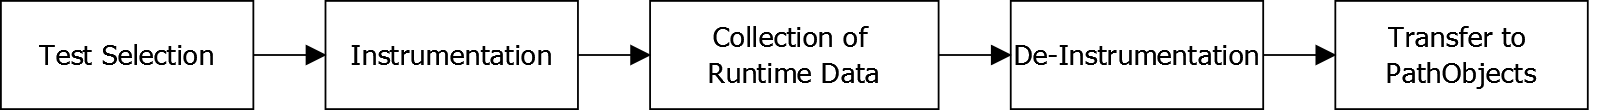
\includegraphics[width=0.9\textwidth]{../images/04-Tracing}
	\caption[TOC Caption]{Tracing foo}
	\label{fig:ImplementationTracing}
\end{figure}

\subsubsection{Shallow Analysis}

Figure \ref{fig:ImplementationTracing} depicts the fundamental steps that are performed by the \textsc{PathTools} tracing framework to generate an execution trace.
First, the user selects a test case of interest that should be traced and visualized.
For instance, this selection can be done through the list of test coverage information that is displayed next to methods in the source browser provided by the \textsc{PathTools} framework.
A \inlinecode{Tracer} object is generated which subsequently initiates the instrumentation phase.
Each method covered by the selected test case is replaced by a \inlinecode{MethodWrapper} that contains the fundamental tracing functionalities.
Thereby, only those methods are regarded that lie within the user-defined tracing scope, i.e. are a member of one of the packages the user selected for tracing.

Method wrappers \cite{brant_wrappers_1998} offer a convenient way to intercept the execution of specific methods.
As the name suggests, they wrap instances of \inlinecode{CompiledMethod} and take their place in the method dictionary of the corresponding class.
They can be utilized to execute code before and after the invocation of the wrapped method.
Furthermore, they allow the inspection and manipulation of arguments as well as of the return value of a message send.
Thereby, the operation of method wrappers is fully transparent for the callers of wrapped methods.

Afterwards, the tracer executes the specified test case.
Since all methods of interest are instrumented at this stage, they automatically report their execution to the tracer.
As method entry and exit events are recorded, a call tree of the selected test case can be constructed.

Once the execution of the test case finishes, the tracer triggers the de-instrumentation phase.
The previously created method wrappers are removed from the method dictionaries and the wrapped compiled methods are put back into their original places.

Finally, the collected information can be converted to a \textsc{PathObjects} trace, which resembles a sequential representation of the execution rather than a tree structure.

\subsubsection{Refinement Runs}
Conceptually, refinement runs are very similar to the shallow analysis process.
The differences are that no test case has to be selected, since the tracer already has a reference to the covered test case.
Furthermore, only those methods are instrumented that are actually required to collect the data that should be refined.
For instance, if the developer queries the state of an argument for a specific message send, only this method is instrumented.
Afterwards, the test is executed again and the installed method wrapper verifies if the current message send is the one the developer specified.
If this is the case, the state of this argument is recorded and reported to the tracer.
Once the test is finished, all method wrappers are removed, and the trace visualization can be updated with the refined information.

The fundamental prerequisite of this strategy is that test cases are strictly deterministic (cf. Section \ref{ss:DiscussionLimitationsTestQuality}).
Otherwise, the returned information might not be related to the developer's query.
For instance, the state of a different object might be returned when a method is called with different arguments in repeated executions.
Additionally, non-deterministic branching that yields a diverging call tree could have the consequence that the refinement run never reaches the specified point of the execution.

\section{Modeling of Objects, States, and Interactions}
\label{s:BackgroundModeling}

\subsection{Object Diagrams}
\label{ss:BackgroundModelingObject}

\begin{figure}
	\centering
	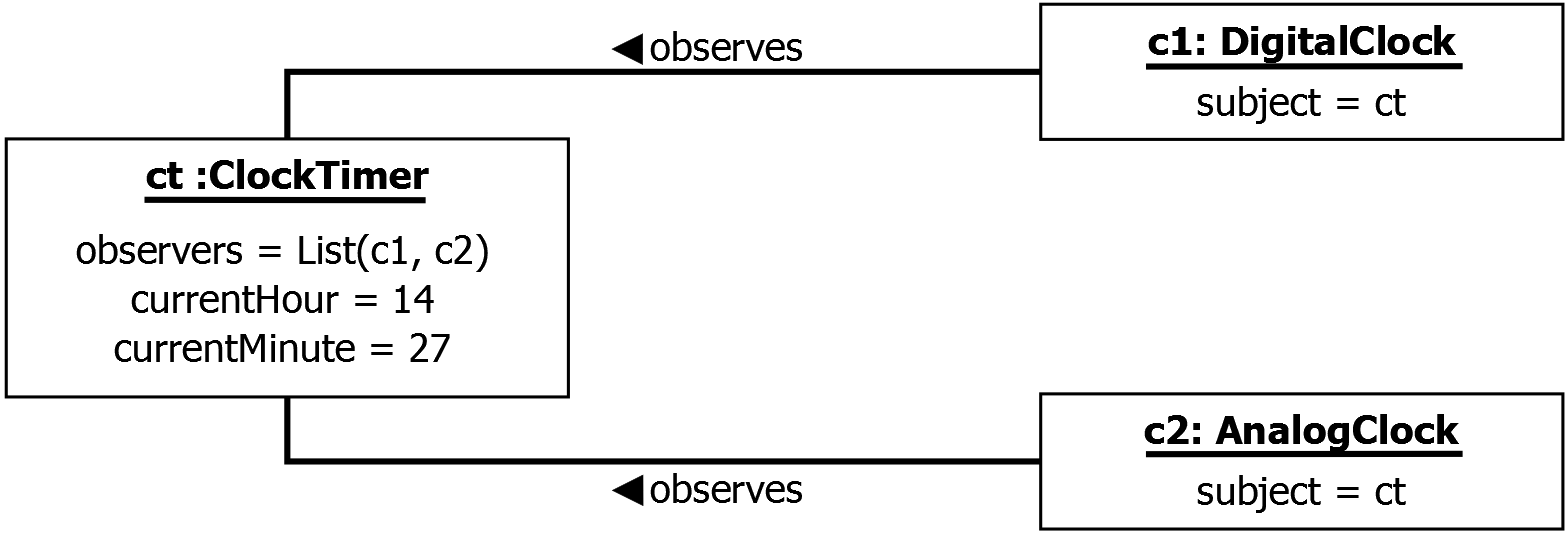
\includegraphics[width=0.7\textwidth]{../images/02-Object}
	\caption[TOC Caption]{UML Object Diagram}
	\label{fig:ModelingObject}
\end{figure}

Object diagrams \cite{rumbaugh_unified_2010} are structural diagrams that can be seen as concretization of a class diagram for a definite point in time.
As such, their notation (cf. Figure \ref{fig:ModelingObject}) covers instances and their state as well as links between instances.
The description of an instance includes an optional identifier, the type of the instance, and a list of attributes and their values.
Links can be annotated with roles and link names, whereby the latter are equipped with indicators for the reading direction.
In addition, links can be declared as forward-navigable and non-backward navigable.

Object diagrams allow the diagram creator to place objects freely on the two-dimensional canvas.
This has the advantage that objects that are closely related can be depicted in spatial proximity.
Likewise, groups of objects that are not related can be placed in different parts of the canvas.
Thus, a map of the system's runtime structure can be created that allows the observer to intuitively get an understanding of the parts of a system and their connections.

\subsection{Sequence Diagrams}
\label{ss:BackgroundModelingSequence}

\begin{figure}
	\centering
	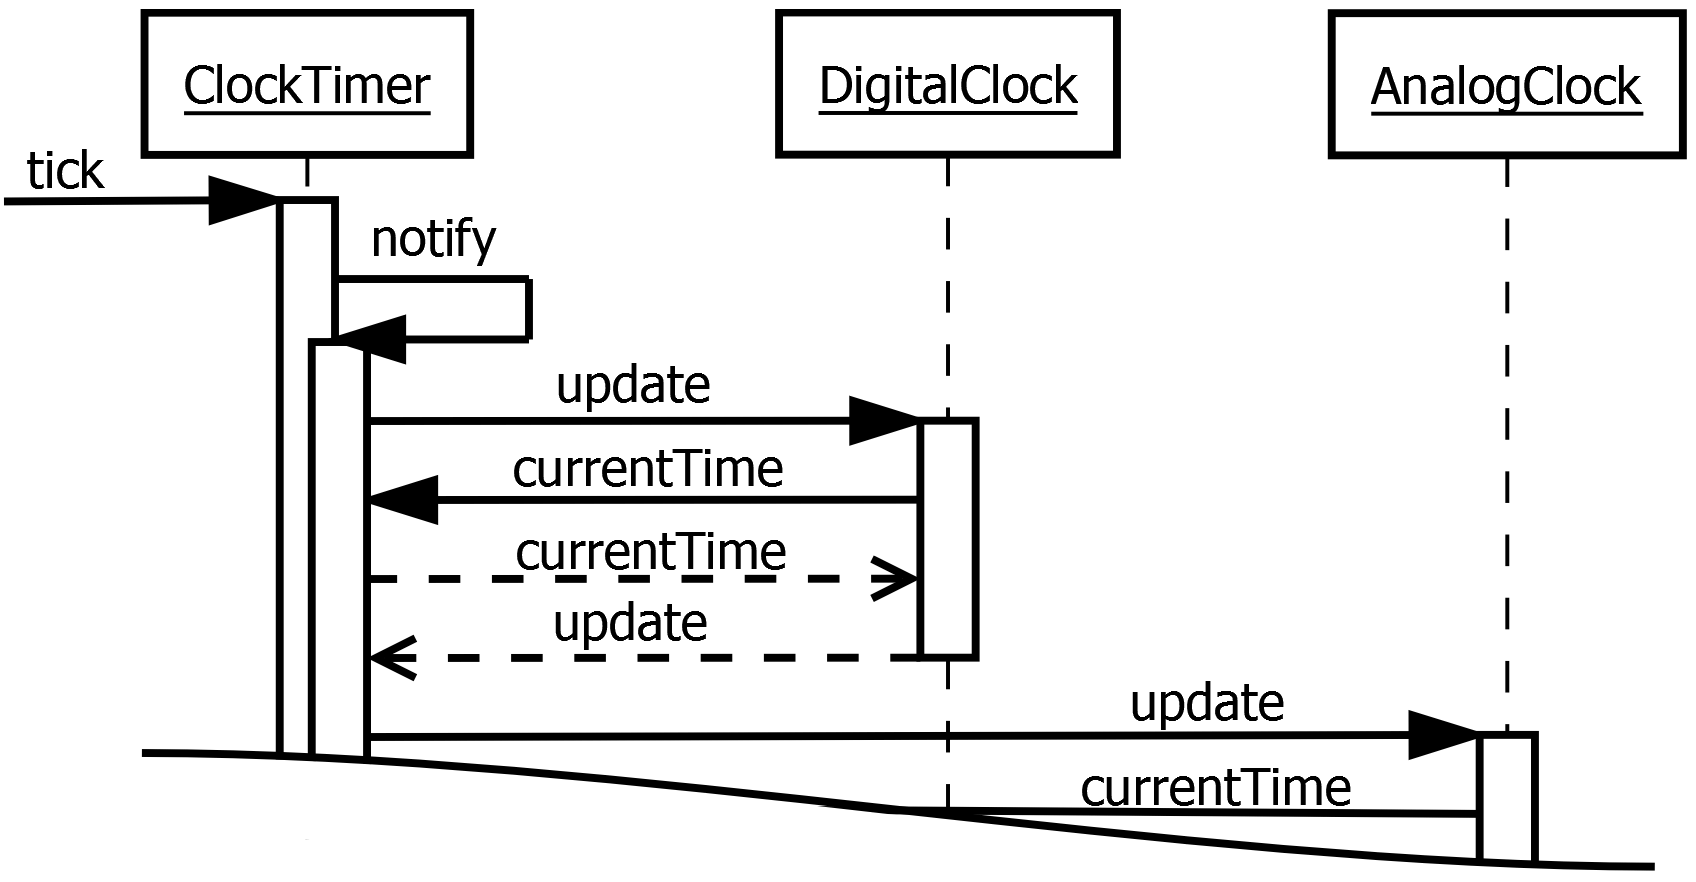
\includegraphics[width=0.6\textwidth]{../images/02-Sequence}
	\caption[TOC Caption]{UML Sequence Diagram}
	\label{fig:ModelingSequence}
\end{figure}

Sequence diagrams \cite{rumbaugh_unified_2010} are used to model the interaction of objects.
Thereby, the focus is on the exchange of messages in a specific scenario rather than the depiction of all possible execution branches.
The fundamental notation elements are depicted in Figure \ref{fig:ModelingSequence}.

Objects and their lifelines are aligned along the horizontal axis.
Execution specifications on the lifelines indicate whether an object is currently participating in a computation.
Messages between two objects are represented by arrows.
They are aligned along the vertical axis according to their chronological appearance.
Each message is complemented by a return message which indicates the end of a method invocation and which is depicted as dashed arrow.
Apart from those basic components, sequence diagrams also can be used to model duration constraints, state invariants and asynchronous behavior.
However, those advanced notation elements are of no great importance in our context.

Sequence diagrams have two major advantages.
Firstly, they feature an inherent chronological ordering, which makes following the communication thread easier for the observer.
Secondly, the automatic generation of sequence diagrams from execution traces is comparatively trivial and consequently fast, as no computation-intensive layout strategies have to be performed.
One could argue that the arrangement of the objects on the horizontal axis should be adjusted to minimize the distance between objects that exchange messages.
This optimization would certainly introduce computational complexity, but does not seem to be a common practice among the wide range of tools offering the generation of sequence diagrams that are reviewed in the related work section (cf. Chapter \ref{c:relatedwork}).

\subsection{Communication Diagrams}
\label{ss:BackgroundModelingCommunication}

\begin{figure}
	\centering
	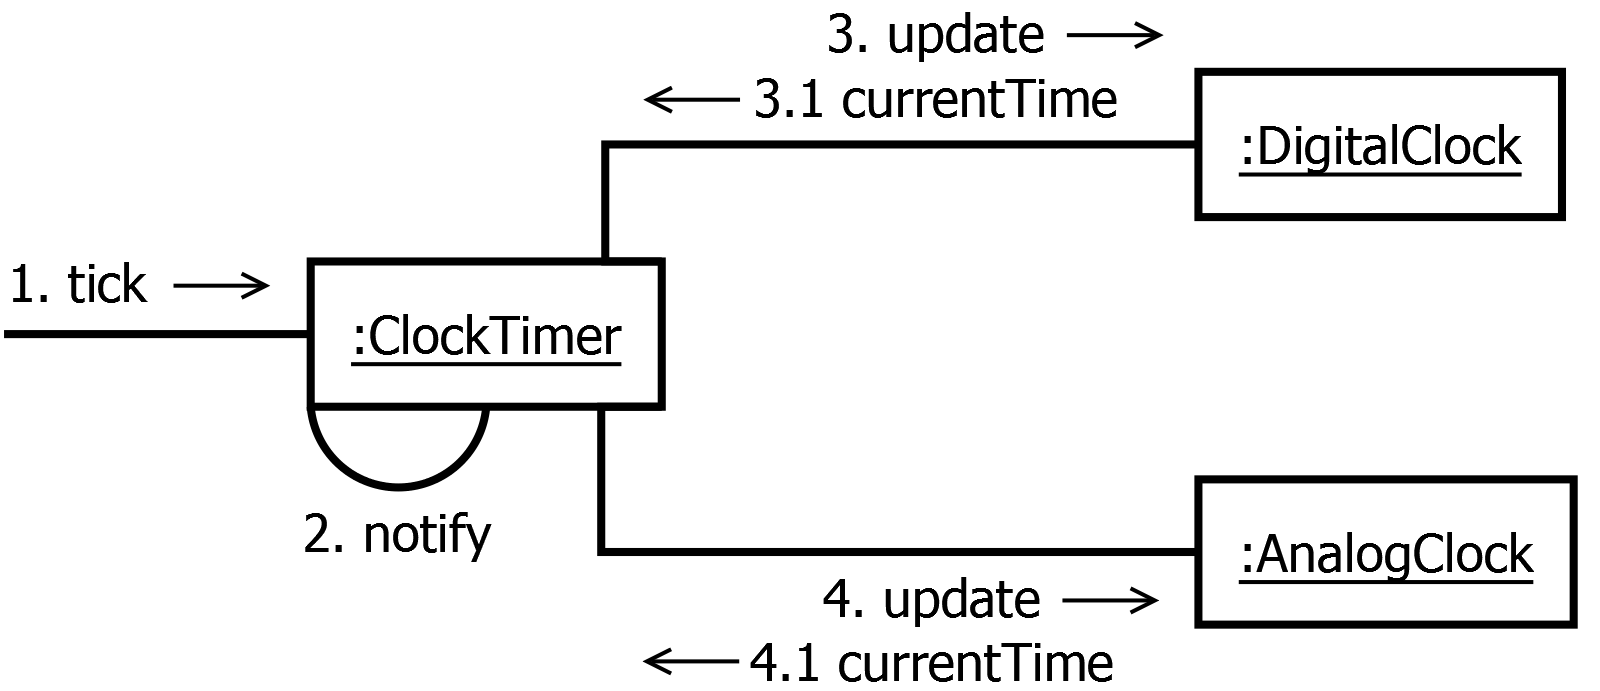
\includegraphics[width=0.6\textwidth]{../images/02-Communication}
	\caption[TOC Caption]{UML Communication Diagram}
	\label{fig:ModelingCommunication}
\end{figure}

Similar to sequence diagrams, communication diagrams \cite{rumbaugh_unified_2010} are used to model the exchange of messages between objects during a specific scenario.
However, the latter rather focus on the relationships between participating objects than on the sequence of exchanged messages.
The notation elements that are used in communication diagrams (cf. Figure \ref{fig:ModelingCommunication}) are similar to the fundamental components of sequence diagrams.
Objects are depicted as lifelines, but everything except the header is omitted.
Objects that are related through message exchanges are connected with an undirected line.
Messages between objects are aligned along those connectors and an orientation indicator shows which object is the sender and respectively the receiver of a message.
Since the notation does not offer an inherent ordering of messages, the sequence is determined through an explicit consecutive hierarchical numbering.

As with object diagrams (cf. Section \ref{ss:BackgroundModelingObject}), the main advantage of communication diagrams lies in the unrestricted placement of objects on the two-dimensional canvas.
It is for this reason that they are often used complementary with sequence diagrams, since the latter are not particularly suitable to communicate which objects belong together in consequence of their communication.

\subsection{Discussion}
Due to the fact that the Unified Modeling Language makes a strict distinction between structural and behavioral diagrams, none of them offers a combined view on object interactions as well as the internal state of objects.
However, to understand the behavior of object-oriented systems, it is important to get an insight into both.
Interactions have to be depicted in order to make the behavior of a system perceivable to the observer.
To understand why a systems behaves the way it does, the internal state of objects has to be unveiled.

Apart from this fundamental problem, the diagrams all have drawbacks of their own that make them inadequate for our objectives.

Sequence diagrams dictate to use one dimension strictly for objects (the horizontal axis) and the second dimension strictly for messages (the vertical axis).
As a result, the extent of such diagrams grows fast and does not scale well with the number of objects and messages that shall be depicted.
Adding objects inevitably leads to an extension of the x-axis, just like adding messages inevitably leads to an extension of the y-axis.
With regard to the extent requirements, it would be much more efficient to allow objects to be placed freely on the canvas, and to route messages between and around objects.
Though our objective is to depict single test cases which are comparatively small units in a software system, they usually still involve dozens of objects and messages respectively.
Scenarios of this magnitude are already sufficient to cause sequence diagrams to grow enormously.
But with the growing size of a diagram, it also becomes increasingly difficult to understand its contents and the relationships between specific components.
In this regard, sequence diagrams do not seem to be the most appropriate choice when it comes down to presenting an execution trace in a manner that is perceivable efficiently.

\section{Challenges}